
%
%  $Description: Author guidelines and sample document in LaTeX 2.09$ 
%
%  $Author: ienne $
%  $Date: 1995/09/15 15:20:59 $
%  $Revision: 1.4 $
%

\documentclass[conference]{IEEEtran}
\usepackage{graphicx,times,amsmath} % Add all your packages here
\usepackage{amsfonts}
%\usepackage{listings}

\usepackage[cp1250]{inputenc}  % or [cp1250], or [latin2], or whatever
                               % suitable for your system


\usepackage{url}


% correct bad hyphenation here
\hyphenation{op-tical net-works semi-conduc-tor IEEEtran}

\IEEEoverridecommandlockouts	% to create the author's affliation portion
				% using \thanks
				
\textwidth 178mm   	% <------ These are the adjustments we made 10/18/2005
\textheight 239mm	% You may or may not need to adjust these numbes again
\oddsidemargin -7mm
\evensidemargin -7mm
\topmargin -6mm 
\columnsep 5mm

\begin{document}

\title{\ \\ \LARGE\bf Fuzzy Classification of Web Reports with Linguistic Text Mining
\thanks{Jan D�dek is with the
Department of Software Engineering, 
Charles University in Prague, Czech Republic 
(email: jan.dedek@mff.cuni.cz).}
\thanks{Peter Vojt� is with the
Institute of Computer Science,
Czech Academy of Sciences and Department of Software Engineering, 
Charles University in Prague, Czech Republic
(email: peter.vojtas@mff.cuni.cz).}
}


\author{Jan D�dek \and Peter Vojt�}


% If the title is too long for the running head, please provide a
% shorter version here:
% (Otherwise leave this command commented out.)
%\titlerunning{Exploitation of linguistic tools in semantic extraction}


% If all authors have the same affiliation do not use the \inst
% command: 
%\author{Jan D�dek\\
%Department of Software Engineering,\\Faculty of Mathematics and Physics,\\
%Department of software engineering\\
%School of Computer Science\\
%Faculty of Mathematics and Physics\\
%Charles University in Prague, Czech Republic\\
%Malostransk� n�m. 25\\
%118 00 Praha 1\\
%Czech Republic\\
%Tel: +420-221-914-264\\
%Fax: +420-221-914-323\\
%Email: jan.dedek@mff.cuni.cz\\
%\and 
%Peter Vojt�\\
%Institute of Computer Science\\
%Academy of Sciences of the Czech Republic\\
%Department of software engineering\\
%School of Computer Science\\
%Faculty of Mathematics and Physics\\
%Charles University in Prague\\
%Malostransk� n�m. 25\\
%118 00 Praha 1\\
%Czech Republic\\
%Tel: +420-221-914-239\\
%Fax: +420-221-914-323\\
%Email: vojtas@cs.cas.cz}


\maketitle              % typesets the title of the contribution

\thispagestyle{empty}



\begin{abstract}
In this paper we present a fuzzy system which increases automation of fuzzy classification of textual web reports. Our approach is based on usage of third party linguistic analyzer and fuzzy inductive logic programming. Main contributions are formal models, prototype implementation and evaluation of experiments of the whole system. 
\end{abstract}

% no key words

\section{Introduction}

General intro

{\bf Priklad}

\begin{figure}[hb!]
\centerline{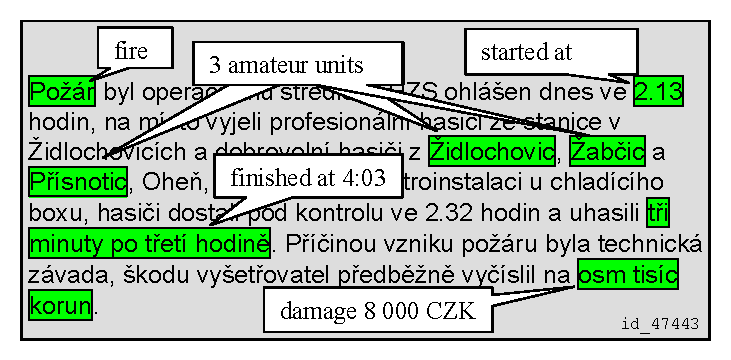
\includegraphics[width=\hsize]{img/message}}
\caption{Example of analyzed web report.}
\label{img:message}
\end{figure}

Problem

Contribution

Related work

more on text mining, information extraction, fuzzy internet applications, ...

In \cite{biblio:YagerReformat08text} 

Paper is organized as follows ...


%%%%%%%%%%%%%%%%%%%%%%%%%%%%%%%%%%%%%%%%%%%%%%%%%%%%%%%%%%%%%%%%%%%%%%%%%%%%%%%%%%%%%%%%%%%%%%%%%
\section{Models, methods, design of the system}
%%%%%%%%%%%%%%%%%%%%%%%%%%%%%%%%%%%%%%%%%%%%%%%%%%%%%%%%%%%%%%%%%%%%%%%%%%%%%%%%%%%%%%%%%%%%%%%%%

\begin{figure}[hb!]
\centerline{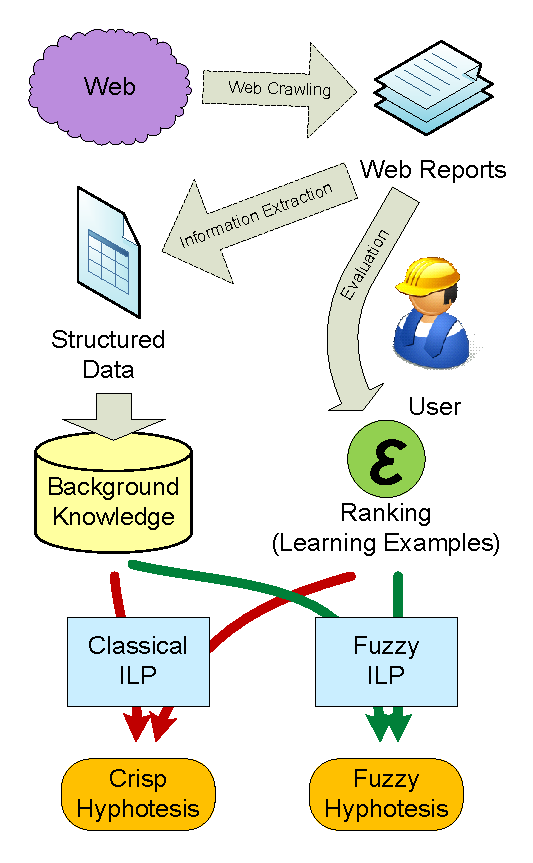
\includegraphics[width=.7\hsize]{img/schema}}
\caption{Schema of presented work (text part).}
\label{img:schema}
\end{figure}

\subsection{Linguistic Analyser}

Citace tectogrammatical structure \cite{biblio:MiBeAnnotationtectogrammatical2006}

\begin{figure}[hb!]
\centerline{\framebox{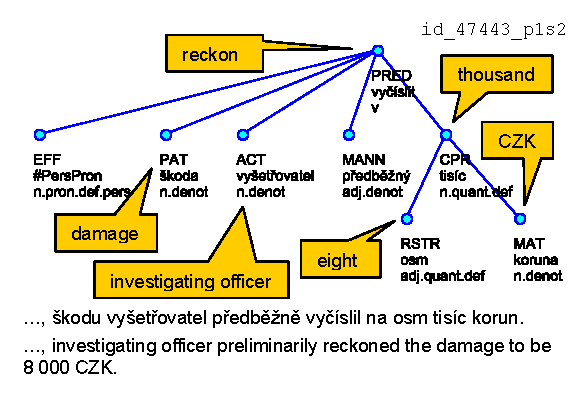
\includegraphics[width=\hsize]{img/tree}}}
\caption{Example of linguistic tree of one of analyzed sentences.}
\label{img:tree}
\end{figure}





\subsection{Classical ILP}

In our application we are facing the challenge of induction and/or mining on several places. First we need an inductive procedure when extracting from web texts attributes of an accident. 

Second we need an inductive procedure when trying to explain degree of seriousness of an accident by attributes of this accident (also called background knowledge).

Both places where induction has to be used have following requirements


\begin{itemize}
	\item data are/can be fuzzy
	\item background knowledge is multirelational
	\item classification is fuzzy
\end{itemize}

Having in mind these requirements we chose Fuzzy inductive logic programming. To make the paper readable we present bellow short description of ILP techniques.

In our presentation of Inductive Logic Programming (ILP) we follow the book of S. D\v zeroski and N. Lavra\v c \cite{dzeroski2001:relat_dm}. Citace ILP \cite{biblio:Muggleton94inductivelogic}

Given is a set of examples $E=P\cup N$, where $P$ contains positive and $N$ negative examples, and a background knowledge $B$. The task is to find a hypothesis $H$ such that 

$$
(\forall e\in P)(B\cup H\models e)
$$
and
$$
(\forall e\in N)(B\cup H\not\models e).
$$
Typically, $E$ consists of ground instances of the target predicate which has to be classified - in our case accidents. $B$ typically consists of several predicates (relational tables) which describe properties of object which have to be classified - in our case properties of accidents. Background knowledge can contain also some rules. Hypothesis $H$ typically consists of logic programming rules, which when added to $B$, explain all positive examples and no negative examples.

Main advantage of ILP is it's multirelational character, namely $B$ can reside in several tables.



\subsection{Fuzzy and GAP induction}

In our presentation of Inductive Logic Programming (ILP) we follow the Paper of T. Horvath and P. Vojtas \cite{biblio:FILP} about fuzzy inductive logic programming. Citace Fuzzy ILP \cite{biblio:FILP}

We use the approach of the fuzzy logic in narrow sense developped by J. Pavelka and P. Hajek. Formulas are of the form $\varphi, x$ ($\varphi$ is syntactically same as in the crisp case) are graded by a truth value $xin [0,1]$.
A structure ${\mathcal M}$ consist of domain $M$ and relations are interpreted fuzzy (we do not consider function symbols here). Evaluation $\left\|\varphi\right\|_{{\mathcal M}}$ of a formula $\varphi$ uses truth functions of many valued connectives (our logic is extensional and/or truth functional). Satisfaction is defined by
$$
{\mathcal M}\models_f (\varphi, x)\ iff\ \left\|\varphi\right\|_{{\mathcal M}}\ge x
$$


Given is a fuzzy set of examples ${\mathcal E}:E\longrightarrow [0,1]$ and a fuzzy background knowledge ${\mathcal B}:B\longrightarrow [0,1]$. The task is to find a fuzzy hypothesis ${\mathcal H}:H\longrightarrow [0,1]$ such that 

$$
(\forall e,f\in dom(E))(\forall {\mathcal M})({\mathcal M}\models_f B\cup H)
$$
we have
$$
E(e)>E(f)\Rightarrow \left\|e\right\|_{{\mathcal M}}\ge \left\|f\right\|_{{\mathcal M}}.
$$

That is, it cannot happen that 
$$
E(e)>E(f) \wedge \left\|e\right\|_{{\mathcal M}}< \left\|f\right\|_{{\mathcal M}},
$$
or rephrased, if $E$ is rating $e$ higher than $f$, then it can not happen in a model of $B\cup H$ that $e$ is rated worse than $f$.

Typically, ${\mathcal E}$ consists of ground instances of the target predicate which are  classified in truth degrees - in our case degree of seriousness of an accident. $B$ typically consists of several fuzzy predicates (fuzzy relational tables) which describe properties of object which have to be classified - in our case fuzzy properties of accidents - degree od injury, degree of damage, .... Background knowledge can contain also some rules, so far only crisp rules are used. Hypothesis $H$ typically consists of a fuzzy logic program, which when added to $B$, prevents of misclassification (better can not be declared to be worse, nevertheless can be declared as having same degree (for more detailed discussion on this definition of fuzzy ILP we reffer to the paper \cite{biblio:FILP})). Moreover, in practise, we use GAP - Generalized Annotated Programs, so graded formulas wil lbe sometimes understood as annotated (with crisp connectives and more complex annotation of head of rules.)

\subsection{Translation of fuzzyILP task to several classical ILP tasks}

As far as there is no implementation of fuzzy (GAP) ILP, we have to use a classical ILP system. Fortunately a fuzzy ILP task can be translated to several crisp ILP tasks (subject to some rounding and using finite set of truth values).

Assume, our fuzzy sets take values for a finite set of truth values $\{0,1\}\subseteq T\subseteq [0,1]$. For each predicate $p(x)$ in $B$ we add an additional attribute for truth value $p(x,t)$. We construct a crisp background knowledge ${\mathcal B}^{mon}_T$ by a process called monotonization, as follows:

If ${\mathcal B}(p(x))=t\in T$, then for all $t'\in T, t'\le t$ we add $p(x,t')\in {\mathcal B}^{mon}_T$.

For all $t\in T$ we create a crisp example set $E_t=P_t\cup N_t$, where
$$
e\in P_t \ \ iff \ \ {\mathcal E}(e)\ge t
$$
and $N_t$ is the rest.

For each $t\in T$ we create a crisp ILP task $E_t, {\mathcal B}^{mon}_T$ and get a hypothesis $H_t$ guaranteeing examples of degree at least $t$. Note that variable boundings ib $B$ have no boundings on truth value attribute, which was added to each predicate, and hence there are no variable boundings in $H$ on truth value attribute. To predicate in $E$ we did not add the additional truth value attribute

Let us assume $C$ is the target predicate in the domain of ${\mathcal E}$. We define ${\mathcal H}$ with domain consisting of one GAP rule 
$$
C(y):u(x_1,\dots,x_m)\leftarrow B_1:x_1 \&\dots\& B_n:x_m,
$$
here $B_1:x_1 \&\dots\& B_n:x_m$ is enumaration of all predicates in $B$.

Assume $B_1(y_1,t_1),\dots,B_n(y_n,t_n)$ are some predicates in $B$ (for simplicity enumerated from 1 to $n\le m$). Then for each rule 
$$
R=C(y)\Leftarrow B_1(y_1,t_1),\dots,B_n(y_n,t_n)
$$
in $H_t$ we give a constraint in definition of $u$ as follows
$$
U_R=u(x_1,\dots,x_m)\ge t \hbox{ if }x_1\ge t_1,\dots,x_n\ge t_n.
$$
Note that $x_{n+1},\dots,x_m$ have no restrictions.

We claim, that if all $H_t$ were correctly learned by an crisp ILP system then for $u$ the minimal solution of all constraints $U_R$ for all $R\in H_t$, for all $t\in T$, the rule
$$
C(y):u(x_1,\dots,x_m)\leftarrow B_1:x_1 \&\dots\& B_n:x_m,
$$
is a correct solution to fuzzy ILP task given by ${\mathcal E}$ and ${\mathcal B}$. Our presentation is here a little bit simplified and we freely switch betwee fuzzy and GAP programs, which are know to be equivalent {\bf citace Krajci, Lencses, Vojtas FSS clanek}

%%%%%%%%%%%%%%%%%%%%%%%%%%%%%%%%%%%%%%%%%%%%%%%%%%%%%%%%%%%%%%%%%%%%%%%%%%%%%%%%%%%%%%%%%%%%%%%%%
\section{The system prototype and Setting of our experiment}
%%%%%%%%%%%%%%%%%%%%%%%%%%%%%%%%%%%%%%%%%%%%%%%%%%%%%%%%%%%%%%%%%%%%%%%%%%%%%%%%%%%%%%%%%%%%%%%%%
The main experiment presented in this paper leads to the seriousness classification of an accident presented on a web report. Our long term goal is extraction of semantic information from web reports. And seriousness classification is one of possible utilization of the extracted semantic information. We use web reports of fire departments of several regions of the Czech Republic. These reports are written in Czech language and can be accessed through the web of General Directorate of the Fire and Rescue Service of the Czech Republic\footnote{\url{http://www.hzscr.cz}}. These reports are rich in information, e.g. where and when an traffic accident occurred, which units helped, how much time it took them to show up on the place of accident, how many people were injured, killed etc.

For the present experiment we have selected a collection of 50 web reports. We have identified several features presented in these reports and manually extracted corresponding values. This will be described in more detail in section \ref{sec:features}. To each report we have also assigned a value of overall ranking of seriousness of presented accident, which is the target of the classification.

\textbf{M�me dv� mo�nosti -- bu� odk�zat na na�e p�edchoz� �l�nky o extrakci informac� nebo se pokusit sem n�co d�t...}


There are two objectives to do. Fist is the web information extraction, a long path starting with web crawling and resulting with the extracted structured information. Second is the seriousness classification, which utilizes the extracted information. We have made much work on the first (see e.g. \cite{biblio:DeVoLinguisticextraction2008,biblio:DeVoComputingaggregations2008, biblio:DeEcExperimentswith2008}), in this paper we will concentrate on the second.



%%%%%%%%%%%%%%%%%%%%%%%%%%%%%%%%%%%%%%%%%%%%%%%%%%%%%%%%%%%%%%%%%%%%%%%%%%%%%%%%%%%%%%%%%%%%%%%%%
\subsection{Experiment description} \label{sec:experiment_desc}
%%%%%%%%%%%%%%%%%%%%%%%%%%%%%%%%%%%%%%%%%%%%%%%%%%%%%%%%%%%%%%%%%%%%%%%%%%%%%%%%%%%%%%%%%%%%%%%%%

For the seriousness classification we have used two inductive logic approaches -- Classical ILP and Fuzzy ILP (as described above). Technically the difference between the approaches consist in different setting of \emph{ILP task}. Both can be done with a classical ILP tool. We have used 
``\emph{A Learning Engine for Proposing Hypotheses}'' (Aleph  v5\footnote{\url{http://www.comlab.ox.ac.uk/activities/machinelearning/Aleph/}}), which seems very practical to us. It use quite effective method of \emph{inverse entailment} \cite{biblio:InverseEntailment} and keeps all handy features of Prolog system (supports YAP and SWI) in its background.

We have compared results of the two approaches (fuzzy and classical) and we could see that the fuzzy approach made better results than the classical one. See section \ref{sec:results} for details of the results.




%%%%%%%%%%%%%%%%%%%%%%%%%%%%%%%%%%%%%%%%%%%%%%%%%%%%%%%%%%%%%%%%%%%%%%%%%%%%%%%%%%%%%%%%%%%%%%%%%
\subsection{Features of accidents} \label{sec:features}
%%%%%%%%%%%%%%%%%%%%%%%%%%%%%%%%%%%%%%%%%%%%%%%%%%%%%%%%%%%%%%%%%%%%%%%%%%%%%%%%%%%%%%%%%%%%%%%%%

\begin{figure}
\centerline{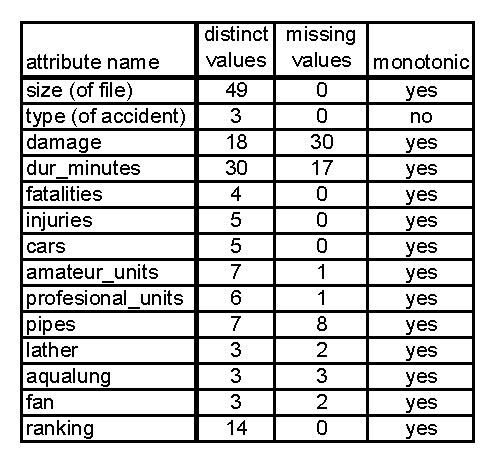
\includegraphics[width=.7\hsize]{img/attributes_description}}
\caption{Characteristics of accident attributes.}
\label{img:attributes_description}
\end{figure}

Figure \ref{img:attributes_description} summarizes all features (or attributes) that we have obtained from accident reports. Except the attribute \verb+type+ (type of an accident -- \verb+fire+, \verb+car_accident+ and \verb+other+) all the attributes are numerical and so monotonizable. In some cases value of some attribute is unknown. We have decided to make evidence of this and keep the values \verb+unknown+ in a knowledge base. Short explanation of each attribute follows.

\verb+size+ is a file size of text part of a report.\\
	\verb+damage+ is an amount (in CZK -- Czech Crowns) of summarized damage arisen during an accident.\\
	\verb+dur_minutes+ is time (in minutes) taken to handle an accident.\\
	\verb+fatalities+ and \verb+injuries+ are numbers of fatalities (and injuries) taken by an accident.\\
	\verb+cars+ is number of cars damaged during an accident (especially during car accidents).\\
	\verb+professional_units+ and \verb+amateur_units+ are numbers of fireman units sent for an accident.\\
	\verb+pipes+ is number of  used fire pipes.\\
	\verb+lather+, \verb+aqualung+ and \verb+fan+ (ventilator) indicates weather these devices were used.

%%%%%%%%%%%%%%%%%%%%%%%%%%%%%%%%%%%%%%%%%%%%%%%%%%%%%%%%%%%%%%%%%%%%%%%%%%%%%%%%%%%%%%%%%%%%%%%%%
\subsection{Seriousness ranking} \label{sec:seriousness}
%%%%%%%%%%%%%%%%%%%%%%%%%%%%%%%%%%%%%%%%%%%%%%%%%%%%%%%%%%%%%%%%%%%%%%%%%%%%%%%%%%%%%%%%%%%%%%%%%

\begin{figure}
\centerline{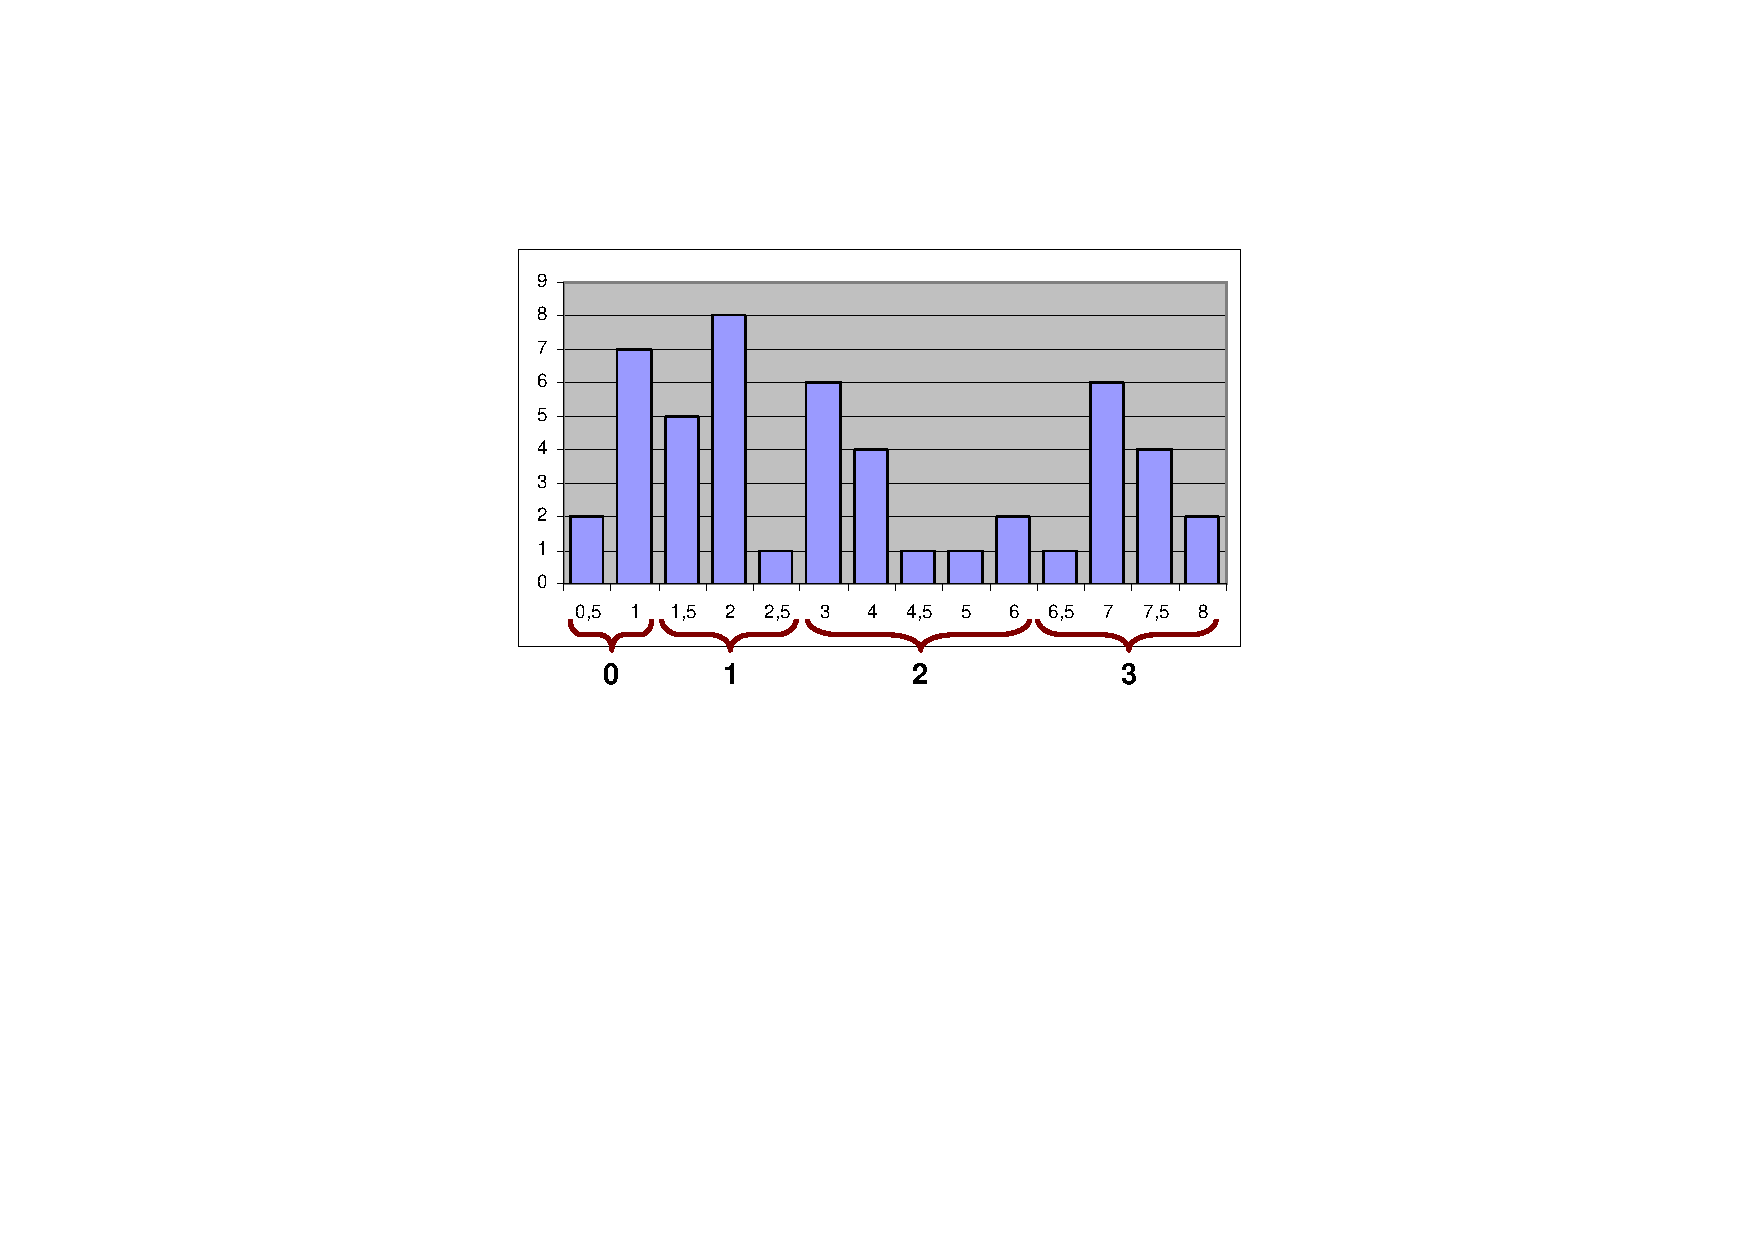
\includegraphics[width=\hsize]{img/ranking_histogram}}
\caption{Frequency histogram of accident ranking.}
\label{img:ranking_histogram}
\end{figure}

Vales of overall seriousness ranking attribute were stated from ``general impression'' from report's texts with respect to the particular attributes (Fig~\ref{img:attributes_description}). Values of seriousness ranking have evolved to 14 distinct values in range form 0.5 to 8. Histogram with frequencies of all the values is on the Figure~\ref{img:ranking_histogram}.

We have divided the values into four approximately equipotent groups (shown on the Fig.~\ref{img:ranking_histogram}) and learned logic rules for each group separately.



%%%%%%%%%%%%%%%%%%%%%%%%%%%%%%%%%%%%%%%%%%%%%%%%%%%%%%%%%%%%%%%%%%%%%%%%%%%%%%%%%%%%%%%%%%%%%%%%%
\section{Results} \label{sec:results}
%%%%%%%%%%%%%%%%%%%%%%%%%%%%%%%%%%%%%%%%%%%%%%%%%%%%%%%%%%%%%%%%%%%%%%%%%%%%%%%%%%%%%%%%%%%%%%%%%


\begin{figure}
\centerline{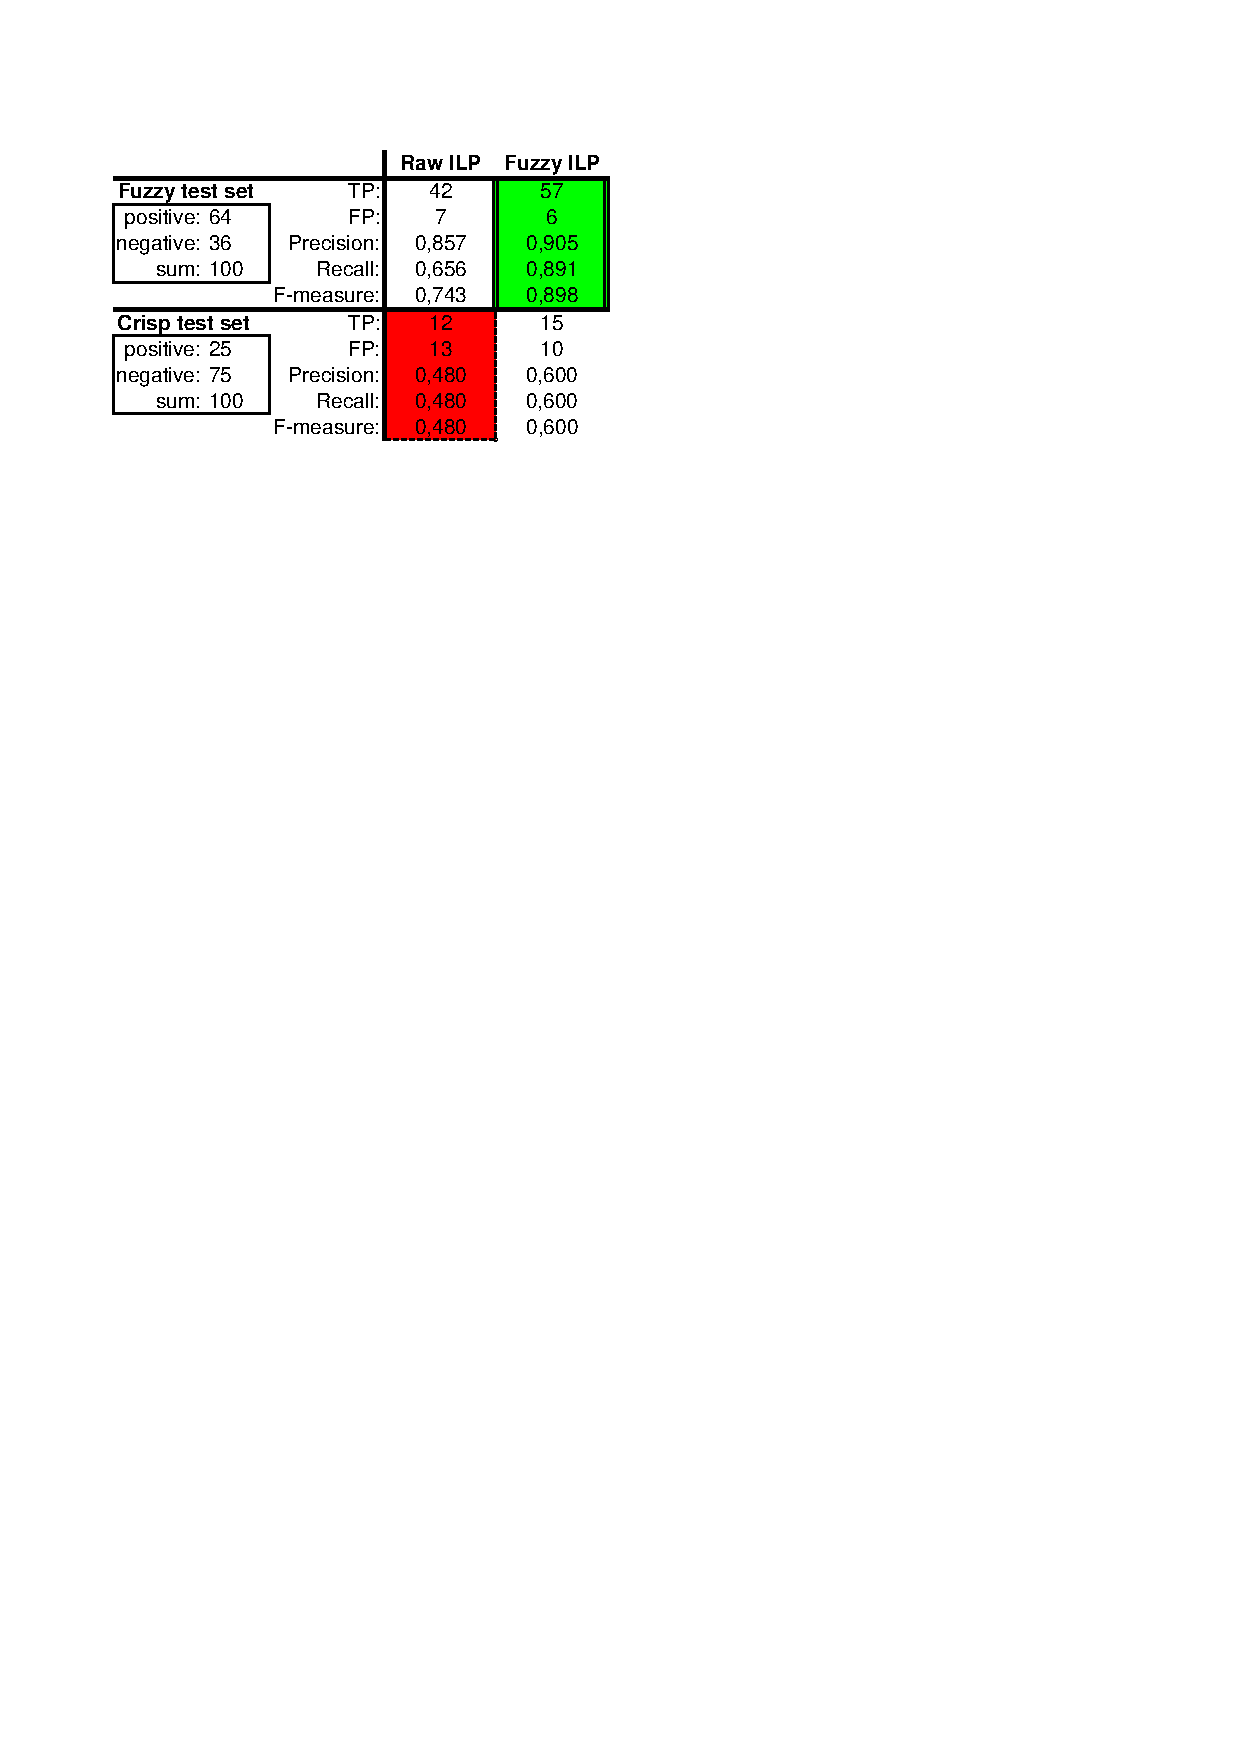
\includegraphics[width=0.8\hsize]{img/Evaluation}}
\caption{Evaluation results}
\label{img:evaluation}
\end{figure}



\begin{figure}
\centerline{
\includegraphics[width=.8\hsize]{img/monot2nomon}}
\caption{Conversion of results: monotone $\rightarrow$ crisp.}
\label{img:monot2nomon}
\end{figure}

\begin{figure}
\centerline{
\includegraphics[width=.8\hsize]{img/nomon2monot}}
\caption{Conversion of results: crisp $\rightarrow$ monotone.}
\label{img:nomon2monot}
\end{figure}

\begin{figure}
\centerline{
\includegraphics[width=.8\hsize]{img/attribute_monotonisation}}
\caption{Monotonization of attributes (damage $\rightarrow$ damage\_atl).}
\label{img:attribute_monotonisation}
\end{figure}



\begin{figure}
\centerline{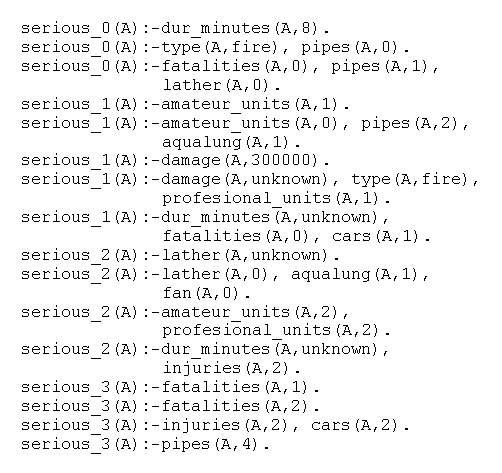
\includegraphics[width=\hsize]{img/rules_nonmonot}}
\caption{Crisp hypothesis}
\label{img:rules_nonmonot}
\end{figure}

\begin{figure}
\centerline{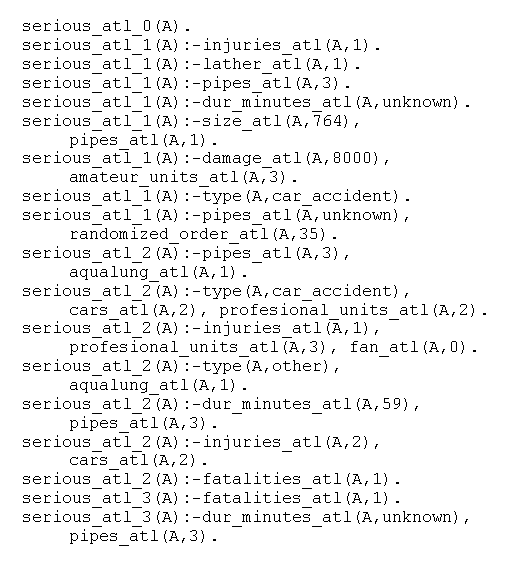
\includegraphics[width=\hsize]{img/rules_monot}}
\caption{Monotonised hypothesis}
\label{img:rules_monot}
\end{figure}

\begin{figure}
\centerline{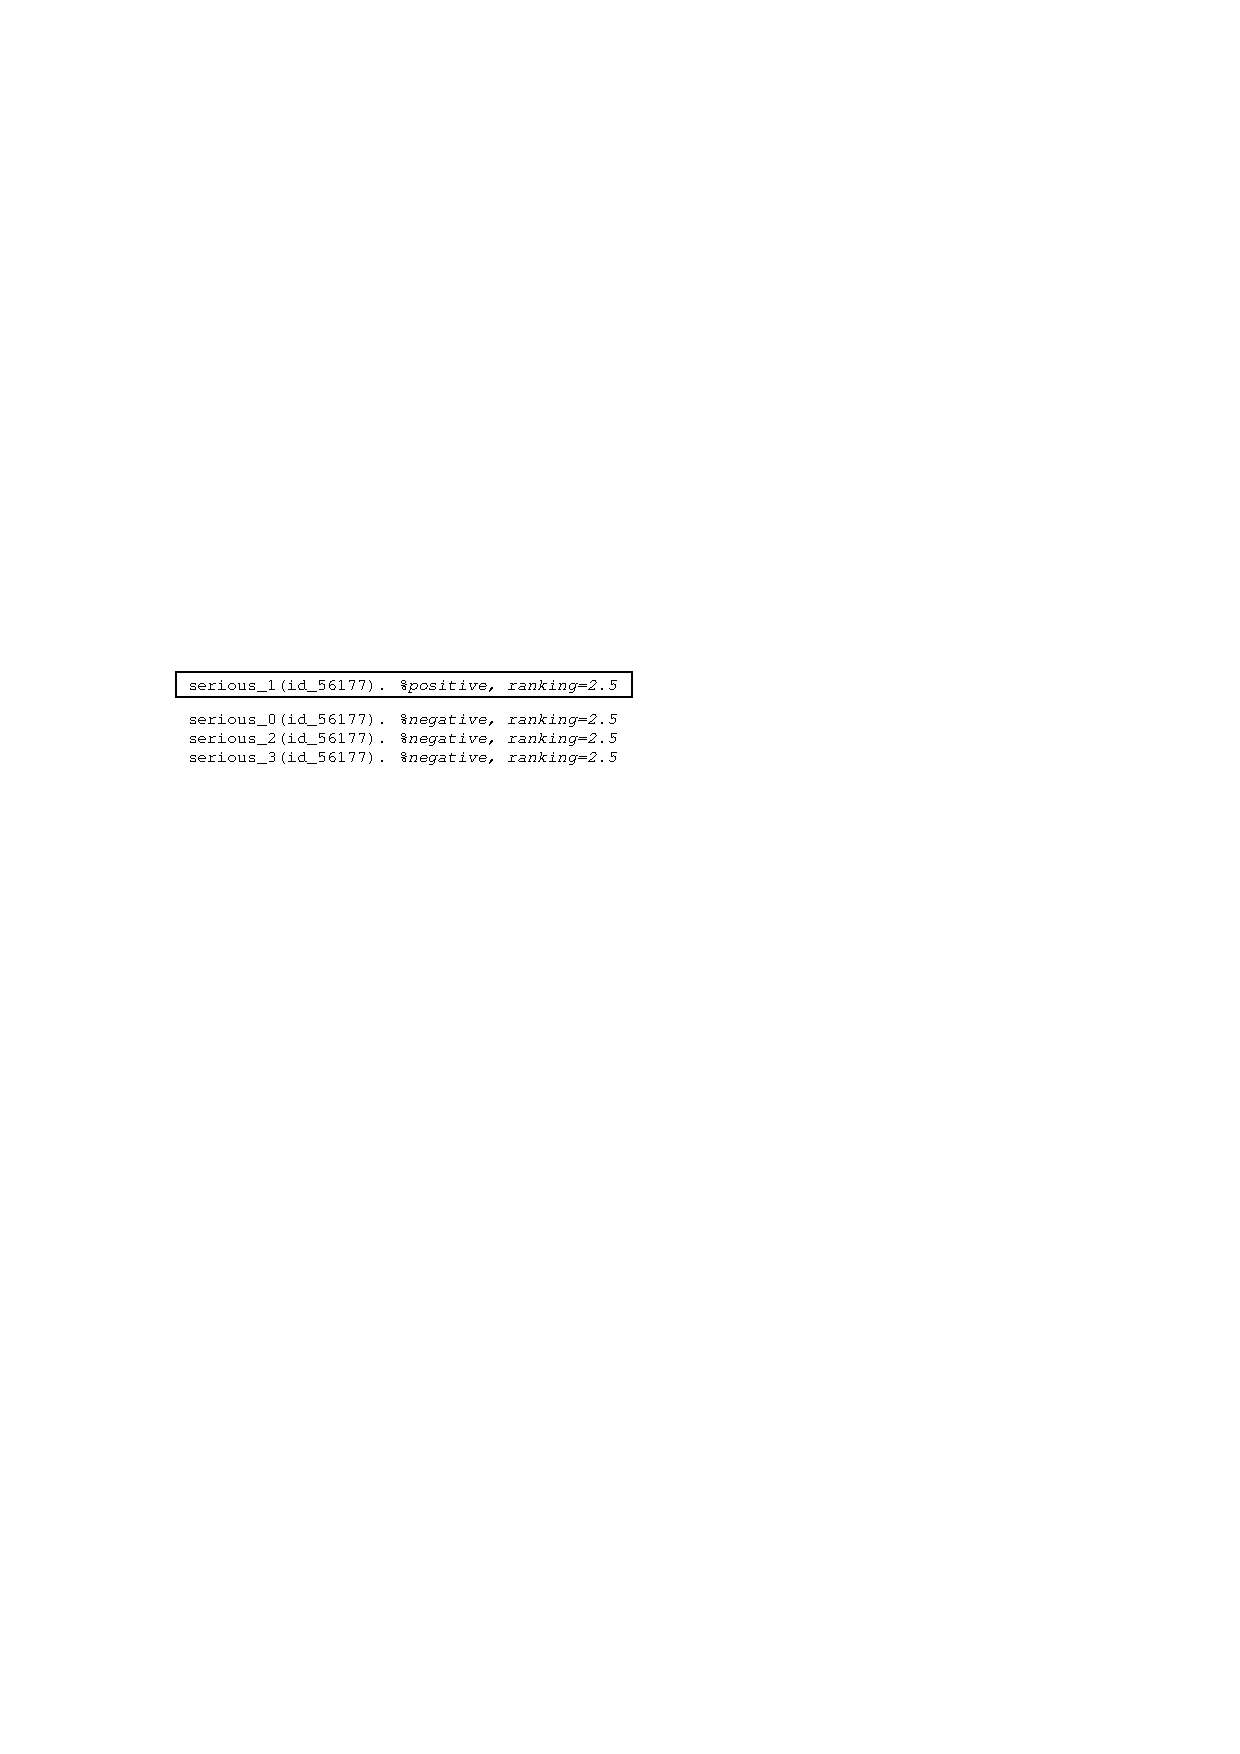
\includegraphics[width=.9\hsize]{img/examples_nonmonot}}
\caption{Crisp learning examples.}
\label{img:examples_nonmonot}
\end{figure}


\begin{figure}
\centerline{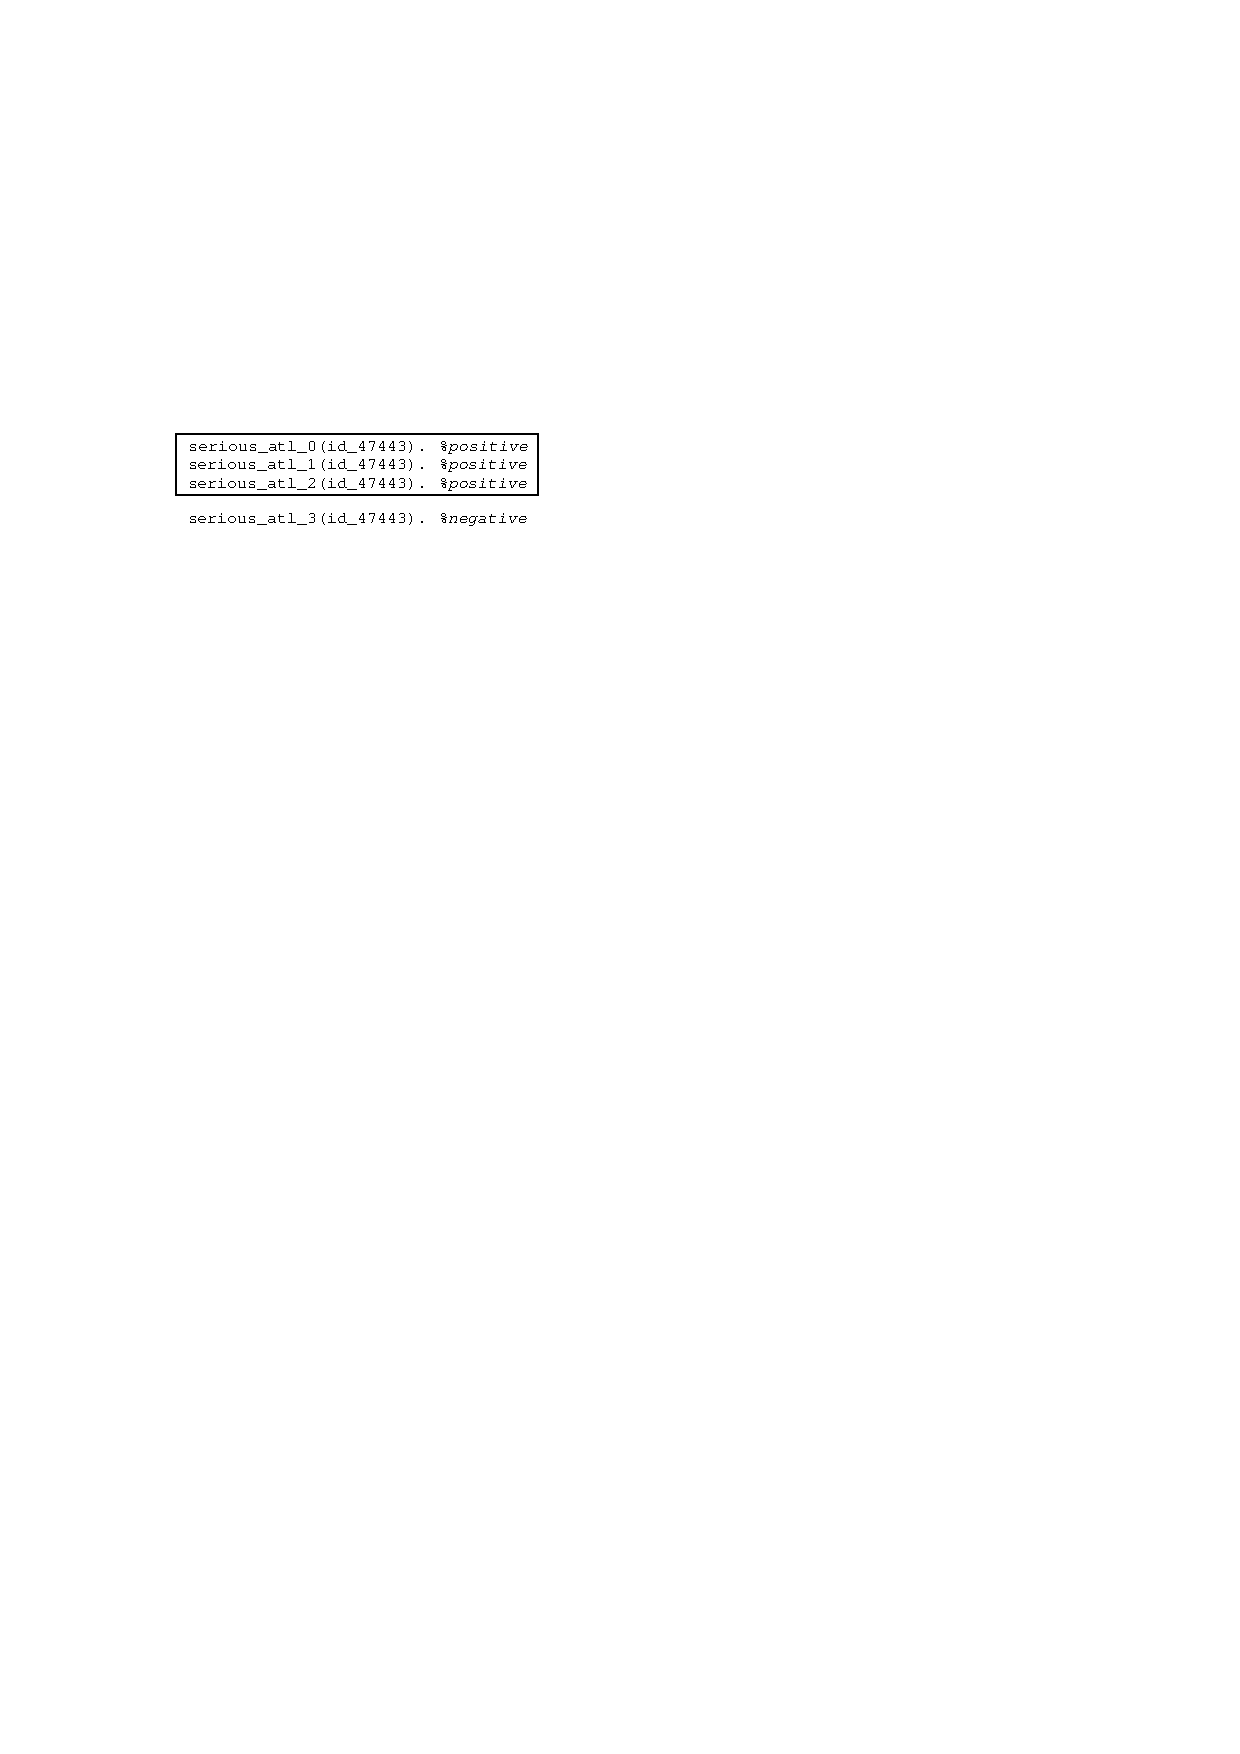
\includegraphics[width=\hsize]{img/examples_monot}}
\caption{Monotonised learning examples.}
\label{img:examples_monot}
\end{figure}



See fig~\ref{img:evaluation}.


%%%%%%%%%%%%%%%%%%%%%%%%%%%%%%%%%%%%%%%%%%%%%%%%%%%%%%%%%%%%%%%%%%%%%%%%%%%%%%%%%%%%%%%%%%%%%%%%%
\section{Conclusion}
%%%%%%%%%%%%%%%%%%%%%%%%%%%%%%%%%%%%%%%%%%%%%%%%%%%%%%%%%%%%%%%%%%%%%%%%%%%%%%%%%%%%%%%%%%%%%%%%%
We have presented a proposal of and experiments with a system for semantic computing of information from Czech text on Web pages. Our system relies on linguistic annotation tools from PDT \cite{biblio:PDT20_CD} and the tree querying tool Netgraph \cite{biblio:MiNetgraphA2006}. Our contributions are an experimental chain of tools that enables semantic computing. In the third phase -- data extraction -- we formulate an inductive logic programming task over linguistically annotated data. Finally we describe transformation of these data to an ontology. Our initial experiments verified used methods and tools.

In future work we would like to test our method on another languages and compare our results with similar solutions. Our work is very close to domain dependent information extraction such as relation and event extraction. These tasks were considered as Semantic Evaluation in the first place in the MUC-6 conference 1995 \cite{biblio:MUC6}. Contemporary results of the ACE competition\footnote{\url{http://www.nist.gov/speech/tests/ace/}} show the difficulty of these problems, which are very close to ours.

\section*{Acknowledgment}
This work was partially supported by Czech projects IS-1ET100300517, GACR-201/09/H057 and MSM-0021620838.



%\bibliographystyle{latex8}
\bibliographystyle{IEEEtran}

\bibliography{DedekVojtas_FuzzIEEE2009}


\end{document}



%%% Local Variables: 
%%% mode: latex
%%% TeX-master: t
%%% End: 
